Experimentos computacionais foram realizados com o objetivo de avaliar a
aplicação da proposta de indexação multidimensional ao MOKP,
através da observação do número de avaliações de solução e do tempo computacional.
Os testes foram divididos em dois grupos visando o contexto
exato e o heurístico respectivamente.
Em ambos os grupos a performance dos algoritmos utilizando a
indexação proposta pela literatura foi comparada à performance utilizando a
indexação multidimensional proposta por este trabalho.

Para o primeiro grupo, que visa analisar a aplicação da proposta no contexto exato,
foi utilizado o algoritmo Bazgan, por ser considerado pela literatura atual como
o algoritmo exato mais eficiente para o MOKP.
As instâncias consideradas neste primeiro grupo foram baseadas nas mesmas
utilizadas pela literatura em \emph{benchmarks} de algoritmos exatos~\cite{bazgan2009, figueira2013algorithmic, correia2018}.

Para o segundo grupo de experimentos, visando analisar a aplicação da proposta
no contexto heurístico, foi utilizada a implementação do SCE para o MOKP, proposta neste trabalho.
Neste segundo grupo, foram consideradas as instâncias utilizadas
pela literatura para \emph{benchmarks} de heurísticas para o MOKP~\cite{zitzler1998multiobjective,zitzler2001spea2, deb2002fast, zhang2007moea, zouache2018cooperative}.

Ambos os conjuntos são compostos por instâncias de 2 e 3 objetivos.
Ambos os algoritmos foram implementados na linguagem C e testados em
máquinas Intel\textsuperscript{\textregistered} Core\textsuperscript{TM} i5-3570 3.40HGz
com 4Gb de RAM com sistema operacional Linux versão 3.19.0 compilados utilizando
GCC versão 7.3.1 com parâmetro de otimização -O3.

\section{Contexto Exato - Algoritmo Bazgan}

Para o contexto exato, este trabalho não utilizou exatamente as mesmas instâncias utilizadas
pelos autores originais por estas não terem sido divulgadas.
As instâncias foram então novamente geradas aleatoriamente seguindo as mesmas regras de
distribuição definidas no trabalho original.

\missingf{Retirei: "Os autores originais foram contactados em seus e-mail porém não houve resposta.". Não fica bem escrever isso 
no texto. Se for questionado, fala oralmente na defesa.

\resp Ok.

}

As instâncias bi-objetivo são divididas em 4 tipos:
\begin{enumerate}
  \item[A)] Aleatórias: $
    p^j_i \in [1, 1000],
    w_i \in [1,1000]$.
  \item[B)] Não-conflitantes: $
    p^1_i \in [111, 1000],\\
    p^2_i \in [p^1_i - 100, p^1_i + 100],\\
    w_i \in [1,1000]$.
  \item[C)] Conflitantes: $
    p^1_i \in [1, 1000],\\
    p^2_i \in [max\{900-p^1_i;1\}, min\{1100-p^1_i, 1000\}],\\
    w_i \in [1,1000]$.
  \item[D)] Conflitantes com pesos correlacionados: $
    p^1_i \in [1, 1000],\\
    p^2_i \in [max\{900-p^1_i;1\}, min\{1100-p^1_i, 1000\}],\\
    w_i \in [p^1_i+p^2_i-200, p^1_i+p^2_i+200]$.
\end{enumerate}
onde $\in [a,b]$ denota uma distribuição uniforme aleatória no intervalo $[a,b]$.
Para todas as instâncias foi atribuído $W=\frac{1}{2}\floor{\sum^n_{k=1} w^k}$.
Para cada tipo e valor de $n$ foram geradas dez instâncias.
Os valores de $n$ utilizados em cada tipo estão descritos na Tabela~\ref{tab:cpu2dim}.
O termo ``conflitante'' refere-se aos valores de $p^j_i$ em cada item:
em instâncias conflitantes, itens com altos valores de $p^1$ tendem a ter
baixos valores de $p^2$ enquanto que itens com baixos valores de $p^1$ tendem a ter
altos valores de $p^2$.
Por sua vez, instâncias não-conflitantes possuem itens cujos valores de $p^j_i$ não possuem
relação com o peso $w_i$,

Devido a este caráter não-conflitante, instâncias do tipo B
tendem a possuir itens com valores de eficiência bastante discrepantes entre si.
Essa discrepância acaba reduzindo a combinação de itens geradores de soluções eficientes,
resultando em conjuntos Pareto de tamanho reduzido.
Por este motivo, as instâncias do tipo B são consideradas mais fáceis.

O aspecto conflitante das instâncias do tipo $D$, por sua vez, dificulta a decisão
de quais itens são mais eficientes que outros, resultando em
muitas boas combinações de solução e, consequentemente, em \paretoset{} aumentados.
Diante disso, as instâncias do tipo $D$ são consideradas mais difíceis.

Para os experimentos com $3$-objetivo considerou-se
a generalização introduzida por~\cite{bazgan2009}
para os tipos $A$ e $C$ e também duas propostas de generalização
para os tipo $B$ e $D$:
\begin{enumerate}
  \item[A)] Aleatórias: $
    p^j_i \in [1, 1000]\\
    w_i \in [1,1000]$
  \item[B)] Não-conflitantes: $
    p^1_i \in [111, 1000],\\
    p^2_i \in [p^1_i - 100, p^1_i + 100],\\
    p^3_i \in [p^1_i - 100, p^1_i + 100],\\
    w_i \in [1,1000]$.
  \item[C)] Conflitantes: $
    p^1_i \in [1, 1000], \;
    p^2_i \in [1, 1001 - p^1_i] \\
    p^3_i \in [max\{900-p^1_i-p^2_i;1\}, min\{1100-p^1_i-p^2_i, 1001-p^1_i\}]\\
    w_i \in [1,1000]$.
  \item[D)] Conflitantes com pesos correlacionados: $
    p^1_i \in [1, 1000]\\
    p^2_i \in [1, 1001 - p^1_i] \\
    p^3_i \in [max\{900-p^1_i-p^2_i;1\}, min\{1100-p^1_i-p^2_i, 1001-p^1_i\}]\\
    w_i \in [p^1_i+p^2_i+p^3_i-200, p^1_i+p^2_i+p^3_i+200]$.
\end{enumerate}

\missingf{Corrigir: ``aplicando-se a regra utilizada no caso bi-objetivo para os ???????,
ou seja,...''

\resp Corrigi.}

Para todas as instâncias foi atribuído $W=\frac{1}{2}\floor{\sum^n_{k=1} w^k}$.
A generalização do tipo $B$ foi proposta definindo-se o valor de $p^3_i$ conforme
a mesma distribuição utilizada para definir $p^2_i$,
mantendo assim os valores de $p^j_i$ não-conflitantes.
A generalização do tipo D foi proposta aplicando-se para $p^3_i$ a mesma regra de generalização
aplicada no tipo C e, para os pesos, aplicando-se a regra utilizada no caso bi-objetivo para Tipo D,
ou seja, $w_i$ tende a ser proporcional à soma dos valores de $p^j_i$.
Para cada tipo e valor de $n$ foram geradas dez instâncias.
Os valores de $n$ utilizados em cada tipo estão descritos na Tabela~\ref{tab:cpu3dim}.
A utilização da \kdtree{} foi comparada à utilização da árvore AVL,
por ser a estrutura de dados utilizada na proposta original para o algoritmo Bazgan.

%Visto que o objetivo dos experimentos é comparar a proposta deste trabalho com
%o que há proposto pela literatura,
%a utilização da \kdtree{} será comparada à da árvore AVL no caso bi-objetivo.
%Para o caso 3-objetivo a utilização da \kdtree{} será comparada principalmente à da lista,
%que é estrutura proposta pelos autores do algoritmo para este caso.

A Tabela~\ref{tab:cpu2dim} apresenta a média de tempo de execução em segundos
do algoritmo Bazgan para as instâncias bi-objetivo nos casos de utilização da
árvore AVL e \dtree{2}.
Cada célula refere-se à média das 10 instâncias do respectivo caso.
A coluna $n$ apresenta o número de itens na instância enquanto que a
coluna $\ndcol$ apresenta a média de soluções contidas no conjunto Pareto
das respectivas instâncias.
A última coluna apresenta o \emph{speedup} da utilização da \dtree{2} em relação
a utilização da árvore AVL.
As células em destaque possuem os melhores valores de tempo.

\begin{table}[h]
  \centering
  \begin{tabular}{crr|r|rr}
  \hline
  %%%%%%%%%%%%%%%%%
  %   HEADER
  %%%%%%%%%%%%%%%%%
  \multicolumn{3}{c|}{Instance}
  & AVL tree
  & \multicolumn{2}{c}{\dtree{2}}
    \\
  Type
  & $n$
  & $|ND| $
  & time (s)
  & time (s)
  & speedup
    \\ \hline
\multirow{2}{*}{A}
 &  40 &   38.1 & \textbf{0.06} & \textbf{  0.06} &  1.0 \\
 &  60 &   73.1 &    1.12 & \textbf{  0.88} &  1.3 \\
 &  80 &  125.6 &   19.81 & \textbf{ 11.89} &  1.7 \\
 & 100 &  180.4 &  165.24 & \textbf{ 76.50} &  2.2 \\
 & 120 &  233.9 &  708.53 & \textbf{361.87} &  2.0 \\ \hline
\multirow{2}{*}{B}
 & 100 &    3.1 & \textbf{  0.02} &    0.08 &  0.3 \\
 & 200 &   10.0 & \textbf{  0.80} &    5.09 &  0.2 \\
 & 300 &   24.9 & \textbf{  9.45} &   88.30 &  0.1 \\
 & 400 &   36.2 & \textbf{ 95.39} &  730.04 &  0.1 \\
 & 500 &   53.7 & \textbf{255.57} & 2824.65 &  0.1 \\
 \hline
\multirow{2}{*}{C}
 &  20 &   36.6 & \textbf{0.00} & \textbf{   0.00} &  1.0 \\
 &  40 &  102.8 &    0.65 & \textbf{   0.42} &  1.5 \\
 &  60 &  231.9 &   28.98 & \textbf{  14.09} &  2.1 \\
 &  80 &  358.0 &  564.10 & \textbf{ 241.54} &  2.3 \\
 & 100 &  513.8 & 3756.57 & \textbf{1605.19} &  2.3 \\ \hline
\multirow{2}{*}{D}
 &  20 &  174.9 &    0.15 & \textbf{   0.12} &  1.3 \\
 &  30 &  269.3 &   16.82 & \textbf{   7.60} &  2.2 \\
 &  40 &  478.0 &  395.76 & \textbf{ 186.67} &  2.1 \\
 &  50 &  553.4 & 2459.48 & \textbf{1417.94} &  1.7 \\ \hline
\end{tabular}

  \caption{Tempo computacional médio do algoritmo Bazgan para instâncias bi-objetivo.}
  \label{tab:cpu2dim}
\end{table}

Segundo a Tabela~\ref{tab:cpu2dim} observa-se que a \dtree{2} já foi capaz de oferecer
redução no tempo computacional, com speedup de até $2.3$.
Exceto para as instâncias do Tipo B,
cujos tempos foram 3 a 10 vezes maior que quando utilizando a árvore AVL.
Isto se deve ao menor tamanho dos conjuntos Pareto para este tipo de instância,
o que degrada a performance da \dtree{2} devido ao \emph{overhead} da estrutura.
Vale rememorar que, neste algoritmo, o conjunto Pareto é construído de forma incremental
durante a execução das iterações, portanto, a quantidade de soluções guardadas
durante as primeiras iterações são ainda menores que $\ndcol$.
Ainda é possível observar na Tabela~\ref{tab:cpu2dim} o reduzido tamanho do
\paretoset{} para instâncias do tipo B, cuja média é de $3.1$ para o caso de $100$ itens,
sendo esta mesma média no mínimo $180.4$ para os outros tipos de instâncias.

\missingf{Lista??? AVL, certo? na frase ``... 3 a 10 vezes maior que quando utilizando a lista.'' Favor corrigir.

\resp Corrigi.}

A Figura~\ref{fig:cmp2dim} apresenta o número médio de avaliações de soluções
demandado pelo algoritmo para as instâncias bi-objetivo quando
utilizada a árvore AVL (coluna escura) e \dtree{2} (coluna clara).
O eixo horizontal corresponde ao número de itens.
O eixo vertical representa o número de avaliações em escala logarítmica.

\begin{figure}[]
  \centering
\begin{subfigure}{.5\textwidth}
  \centering
  \begin{tikzpicture}
\begin{axis}[
	x tick label style={ /pgf/number format/1000 sep=},
	width=\cmpW, height=\cmpH,
	ylabel=Evaluations,
	ymode=log,
	grid = both,
	grid style={line width=.1pt, draw=gray!10},
	major grid style={line width=.2pt,draw=gray!50},
	%xlabel=Number of items (n),
	enlargelimits=0.15,
	legend style={at={(\legX,\legY)},
		anchor=north,legend columns=-1},
	ybar=2.6pt,% configures `bar shift'
	bar width=9pt,
	point meta=y *10^-7, % the displayed number
	cycle list = {black!80,black!30}
]

\addplot+[fill, text=black]
  coordinates {
    ( 40,3703070)
    ( 60,103534833)
    ( 80,700026931)
    (100,5542292786)
    (120,4935519921)
  };

\addplot+[fill, text=black]
  coordinates {
    ( 40,291655)
    ( 60,1182225)
    ( 80,5434379)
    (100,27996835)
    (120,31578018)
  };

\legend {AVL-tree,\dtree{2}}
\end{axis}
\end{tikzpicture}
  \caption{Type A}
  \label{fig:sub1}
\end{subfigure}%
\begin{subfigure}{.5\textwidth}
  \centering
  
\begin{tikzpicture}
\begin{axis}[
	x tick label style={ /pgf/number format/1000 sep=},
	width=\cmpW, height=\cmpH,
	ylabel=Avaliações,
	ymin=100000,
	ymax=100000000000,
	ymode=log,
	grid = both,
	grid style={line width=.1pt, draw=gray!10},
	major grid style={line width=.2pt,draw=gray!50},
	%xlabel=Number of items (n),
	enlargelimits=0.15,
	legend style={at={(\legX,\legY)},
		anchor=north,legend columns=-1},
	ybar=2pt,% configures `bar shift'
	bar width=8pt,
	xtick={100,200,300,400,500},
	xticklabels={100,200,300,400,500},
	point meta=y *10^-7, % the displayed number
	cycle list = {black!80,black!30}
]

\addplot+[fill, text=black]
  coordinates {
    (100,562886)
    (200,27327963)
    (300,349249789)
    (400,17406619609)
    (500,12137619611)
  };

\addplot+[fill, text=black]
  coordinates {
    (100,330881)
    (200,5329798)
    (300,396002213)
    (400,148865700)
    (500,318904809)
  };

\legend {AVL-tree,\dtree{2}}
\end{axis}
\end{tikzpicture}

  \caption{Type B}
  \label{fig:sub2}
\end{subfigure}
\begin{subfigure}{.5\textwidth}
  \centering
  
\begin{tikzpicture}
\begin{axis}[
	x tick label style={ /pgf/number format/1000 sep=},
	width=\cmpW, height=\cmpH,
	ylabel=Avaliações,
	ymin=100000,
	ymax=100000000000,
	ymode=log,
	grid = both,
	grid style={line width=.1pt, draw=gray!10},
	major grid style={line width=.2pt,draw=gray!50},
	%xlabel=Number of items (n),
	enlargelimits=0.15,
	legend style={at={(\legX,\legY)},
		anchor=north,legend columns=-1},
	ybar=2pt,% configures `bar shift'
	bar width=9pt,
	point meta=y *10^-7, % the displayed number
	cycle list = {black!80,black!30}
]

\addplot+[fill, text=black]
  coordinates {
    ( 20,191729)
    ( 40,18662815)
    ( 60,670819408)
    ( 80,4616460680)
    (100,73868244070)
  };

\addplot+[fill, text=black]
  coordinates {
    ( 20,32950)
    ( 40,926315)
    ( 60,5542258)
    ( 80,23285877)
    (100,80371740)
  };

\legend {AVL-tree,\dtree{2}}
\end{axis}
\end{tikzpicture}

  \caption{Type C}
  \label{fig:sub3}
\end{subfigure}%
\begin{subfigure}{.5\textwidth}
  \centering
  
\begin{tikzpicture}
\begin{axis}[
	x tick label style={ /pgf/number format/1000 sep=},
	width=\cmpW, height=\cmpH,
	ylabel=Avaliações,
	ymin=100000,
	ymax=100000000000,
	ymode=log,
	grid = both,
	grid style={line width=1.3pt, draw=gray!00},
	major grid style={line width=.2pt,draw=gray!50},
	%xlabel=Number of items (n),
	enlargelimits=0.15,
	legend style={at={(\legX,\legY)},
		anchor=north,legend columns=-1},
	ybar=2pt,% configures `bar shift'
	xmin=18,
	xmax=52,
	bar width=9pt,
	point meta=y *10^-7, % the displayed number
	cycle list = {black!80,black!30}
]

\addplot+[fill, text=black]
  coordinates {
    ( 20,2831448)
    ( 30,489772231)
    ( 40,9316773179)
    ( 50,19581372744)
  };

\addplot+[fill, text=black]
  coordinates {
    ( 20,173245)
    ( 30,3317384)
    ( 40,14262798)
    ( 50,57959241)
  };

\legend {AVL-tree,\dtree{2}}
\end{axis}
\end{tikzpicture}

  \caption{Type D}
  \label{fig:sub4}
\end{subfigure}
  \caption{Número de avaliações médio do algoritmo Bazgan para instâncias bi-objetivo.}
  \label{fig:cmp2dim}
\end{figure}

É possível observar na Figura~\ref{fig:cmp2dim} que a utilização da \dtree{2}
reduziu consideravelmente o
número de avaliações de solução, com exceção apenas no caso com $300$ itens do tipo B.
Pode-se notar que, nos casos em que se observou altos valores de speedup
houve grande redução do número de avaliações; em alguns casos obteve-se
uma redução de uma ordem de grandeza.
Vale observar que houve alguma redução no número de avaliações
para o Tipo B, porém não suficiente para reduzir o tempo computacional.
Isto se deve ao reduzido tamanho de seus conjuntos Pareto, para os quais não
se torna vantajoso o \emph{overhead} da \kdtree{}.

A Tabela~\ref{tab:cpu3dim} apresenta a média de tempo de execução em segundos
do algoritmo Bazgan para as instâncias 3-objetivo nos casos de utilização da
árvore AVL, \dtree{2} e \dtree{3}.
Cada célula se refere à média das 10 instâncias do respectivo caso.
A coluna $n$ apresenta o número de itens na instância enquanto que a
coluna $\ndcol$ apresenta a média de soluções contidas no conjunto Pareto
das respectivas instâncias.
As células em destaque possuem os melhores valores de tempo.

\begin{table}[]
  \centering
  \begin{tabular}{crr|r|rc|rc}
  \hline
  %%%%%%%%%%%%%%%%%
  %   HEADER
  %%%%%%%%%%%%%%%%%
  \multicolumn{3}{c|}{Instance}
  & AVL tree
  & \multicolumn{2}{c|}{\dtree{2}}
  & \multicolumn{2}{c}{\dtree{3}}
    \\
  Type
  & $n$
  & $|ND| $
  & time (s)
  & time (s)
  & speedup
  & time (s)
  & speedup
    \\ \hline
  %%%%%%%%%%%%%%%%%
  %   CLASS A
  %%%%%%%%%%%%%%%%%
  \multirow{2}{*}{A}
  & 50 &  557.5 &    41.2 &    21.3 & 1.9 & \textbf{  18.5} & 2.2 \\
  & 60 & 1240.0 &   485.9 &   247.8 & 1.9 & \textbf{  79.9} & 6.0 \\
  & 70 & 1879.3 &  3179.5 &  1038.0 & 3.0 & \textbf{ 614.5} & 5.1 \\
  & 80 & 2540.5 &  6667.9 &  3796.0 & 1.7 & \textbf{2943.9} & 2.2 \\
  & 90 & 3528.5 & 24476.5 & 12916.7 & 1.8 & \textbf{3683.7} & 6.6 \\ \hline
  %%%%%%%%%%%%%%%%
  %   CLASS B
  %%%%%%%%%%%%%%%%%
  \multirow{2}{*}{B}
  & 100 &  18.0 & \textbf{   0.1} &    0.3 & 0.3 &    0.3 & 0.3 \\
  & 200 &  65.4 & \textbf{  11.4} &   34.4 & 0.3 &   29.1 & 0.4 \\
  & 300 & 214.2 & \textbf{ 307.7} &  631.5 & 0.5 &  583.2 & 0.5 \\
  & 400 & 317.0 & \textbf{4492.9} & 8464.9 & 0.5 & 5402.2 & 0.8 \\ \hline
  %%%%%%%%%%%%%%%%%
  %   CLASS C
  %%%%%%%%%%%%%%%%%
  \multirow{2}{*}{C}
  & 20 &  254.4 &   0.06 &   0.05 & 1.2 & \textbf{ 0.03} & 2.17 \\
  & 30 & 1066.6 &   9.69 &   4.18 & 2.3 & \textbf{ 1.30} & 7.46 \\
  & 40 & 2965.5 & 471.68 & 153.21 & 3.1 & \textbf{30.50} & 15.5 \\ \hline
  %%%%%%%%%%%%%%%%
  %   CLASS D
  %%%%%%%%%%%%%%%%%
  \multirow{2}{*}{D}
  & 20 & 4087.7 &   23.6 &   10.9 & 2.2 & \textbf{   1.9} & 12.5 \\
  & 30 & 8834.5 & 8914.2 & 3625.3 & 2.5 & \textbf{1019.5} &  8.7 \\ \hline
\end{tabular}
  \caption{Tempo computacional médio do algoritmo Bazgan para instâncias 3-objetivo.}
  \label{tab:cpu3dim}
\end{table}

Conforme a Tabela~\ref{tab:cpu3dim}, assim como no caso bi-objetivo,
a utilização da \kdtree{} resultou em melhoria
nos tempos computacionais, exceto para as instâncias do Tipo B.
Pode-se observar que o speedup proporcionado pela \dtree{2} para o caso
3-objetivo foi comparável ao caso bi-objetivo.
Porém o speedup resultante da utilização da \dtree{3} foi ainda maior,
especialmente para instâncias difíceis, chegando a alcançar $15.5$.

\missingf{Acho que vc deve explorar mais porque os resultados foram piores no tipo B tanto para bi quanto 3-objetivo.

\resp Ok. Os resultados piores são decorrente do tamanho do conjunto pareto que é minúsculo no caso do tipo B.
Para 100 itens, por exemplo, o tipo B tem tamanho 3, enquanto que nos outros tipo, o mínimo é 180. Comentei isso no texto também.

Também fiz uma discussão sobre o porque do tamanho reduzido do tipo B após a definição das instâncias.
}

A Figura~\ref{fig:cmp3dim} apresenta o número médio de avaliações de soluções
demandado pelo algoritmo para instâncias 3-objetivo quando
utilizada a árvore AVL (coluna direita), \dtree{2} (coluna central)
e \dtree{3} (coluna esquerda).
O eixo horizontal corresponde ao número de itens.
O eixo vertical representa o número de avaliações em escala logarítmica.
É possível observar que a utilização da \dtree{3} reduziu consideravelmente o
número de avaliações de solução, com exceção de um caso do tipo B.
Pode-se notar que, nos casos em que se observou altos valores de speedup
houve grande redução do número de avaliações; em alguns casos obteve-se
uma redução de uma ordem de grandeza.

\begin{figure}[]
  \centering
  \centering
\begin{subfigure}{.5\textwidth}
  \centering
  %\begin{tikzpicture}
\begin{axis}[
	x tick label style={ /pgf/number format/1000 sep=},
	width=\cmpW, height=\cmpH,
	ylabel=Avaliações,
	ymode=log,
	grid = both,
	grid style={line width=.0pt, draw=gray!00},
	major grid style={line width=.2pt,draw=gray!50},
	%xlabel=Number of items (n),
	enlargelimits=0.15,
	legend style={at={(\legX,\legY)},
		anchor=north,legend columns=-1},
	ybar=2pt,% configures `bar shift'
	bar width=7pt,
	point meta=y *10^-7, % the displayed number
	cycle list = {black!80,black!50,black!20}
]

\addplot+[fill, text=black]
  coordinates {
    (50,2557230768)
    (60,1548431035)
    (70,22725915563)
    (80,105604506342)
    (90,243276893280)
  };

\addplot+[fill, text=black]
  coordinates {
    (50,116409692)
    (60,2490816101)
    (70,6444320225)
    (80,40077812473)
    (90,84001331660)
  };
  
\addplot+[fill, text=black]
  coordinates {
    (50,6441918)
    (60,11026583)
    (70,42167703)
    (80,71599151)
    (90,174737779)
  };

\legend {AVL-tree,\dtree{2}, \dtree{3}}
\end{axis}
\end{tikzpicture}

  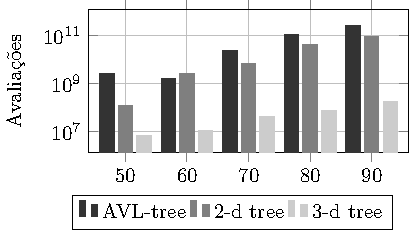
\includegraphics[scale=1.1]{tab/cmp/3dimA}
  \caption{Tipo A}
  \label{fig:sub5}
\end{subfigure}%
\begin{subfigure}{.5\textwidth}
  \centering
  %\begin{tikzpicture}
\begin{axis}[
	x tick label style={ /pgf/number format/1000 sep=},
	width=\cmpW, height=\cmpH,
	ylabel=Evaluations,
	ymode=log,
	grid = both,
	grid style={line width=.0pt, draw=gray!00},
	major grid style={line width=.2pt,draw=gray!50},
	%xlabel=Number of items (n),
	enlargelimits=0.15,
	legend style={at={(\legX,\legY)},
		anchor=north,legend columns=-1},
	ybar=2pt,% configures `bar shift'
	bar width=7pt,
	point meta=y *10^-7, % the displayed number
	cycle list = {black!80,black!50,black!20}
]

\addplot+[fill, text=black]
  coordinates {
    (100,2580591.4)
    (200,367842367.9)
    (300,7975491375.7)
    (400,72030125537.7)
  };

\addplot+[fill, text=black]
  coordinates {
    (100,1571248.6)
    (200,151476739.2)
    (300,2791493175.3)
    (400,45272872459.5)
  };
  
\addplot+[fill, text=black]
  coordinates {
    (100,912878.0)
    (200,29237583.4)
    (300,226471349.8)
    (400,960366212.0)
  };

\legend {AVL-tree,\dtree{2}, \dtree{3}}
\end{axis}
\end{tikzpicture}
  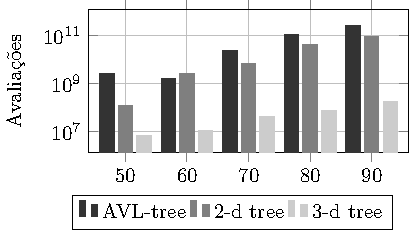
\includegraphics[scale=1.1]{tab/cmp/3dimA}
  \caption{Tipo B}
  \label{fig:sub6}
\end{subfigure}
\begin{subfigure}{.49\textwidth}
  \centering
  %\begin{tikzpicture}
\begin{axis}[
	x tick label style={ /pgf/number format/1000 sep=},
	width=\cmpW, height=\cmpH,
	ylabel=Avaliações,
	ymode=log,
	grid = both,
	grid style={line width=.1pt, draw=gray!00},
	major grid style={line width=.2pt,draw=gray!50},
	%xlabel=Number of items (n),
	enlargelimits=0.15,
	xtick={20, 30, 40},
	xticklabels={20, 30, 40},
	xmin=18,
	xmax=42,
	legend style={at={(\legX,\legY)},
		anchor=north,legend columns=-1},
	ybar=2pt,% configures `bar shift'
	bar width=7pt,
	point meta=y *10^-7, % the displayed number
	cycle list = {black!80,black!50,black!20}
]

\addplot+[fill, text=black]
  coordinates {
    ( 20,221956989)
    ( 30,10861341339)
    ( 40,26505319423)
  };

\addplot+[fill, text=black]
  coordinates {
    ( 20,235426288)
    ( 30,1340276850)
    ( 40,5943925097)
  };
  
\addplot+[fill, text=black]
  coordinates {
    ( 20,1919561)
    ( 30,10225751)
    ( 40,63529280)
  };

\legend {AVL-tree,\dtree{2}, \dtree{3}}
\end{axis}
\end{tikzpicture}

  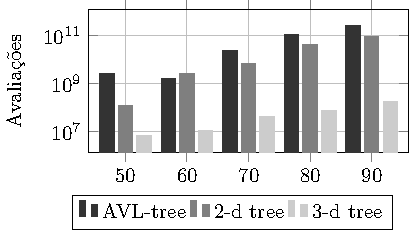
\includegraphics[scale=1.1]{tab/cmp/3dimA}
  \caption{Tipo C}
  \label{fig:sub7}
\end{subfigure}
\begin{subfigure}{.49\textwidth}
  \centering
  %\begin{tikzpicture}
\begin{axis}[
	x tick label style={ /pgf/number format/1000 sep=},
	width=\cmpW, height=\cmpH,
	ylabel=Evaluations,
	ymode=log,
	grid = both,
	grid style={line width=.0pt, draw=gray!00},
	major grid style={line width=.2pt,draw=gray!50},
	%xlabel=Number of items (n),
	enlargelimits=0.15,
	xtick={20, 30},
	xmin=17,
	xmax=33,
	legend style={at={(\legX,\legY)},
		anchor=north,legend columns=-1},
	ybar=2pt,% configures `bar shift'
	bar width=8pt,
	point meta=y *10^-7, % the displayed number
	cycle list = {black!80,black!50,black!20}
]

\addplot+[fill, text=black]
  coordinates {
    (20,481435295.3)
    (30,89269703684.8)
  };

\addplot+[fill, text=black]
  coordinates {
    (20,161607530.0)
    (30,32867842298.12)
  };
  
\addplot+[fill, text=black]
  coordinates {
    (20,2127432.7)
    (30,59136651.9)
  };

\legend {AVL-tree,\dtree{2}, \dtree{3}}
\end{axis}
\end{tikzpicture}
  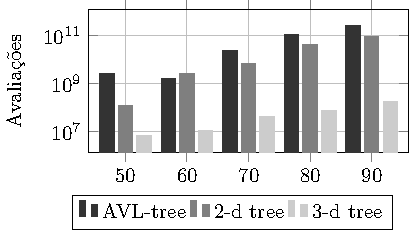
\includegraphics[scale=1.1]{tab/cmp/3dimA}
  \caption{Tipo D}
  \label{fig:sub8}
\end{subfigure}

  \caption{Número de avaliações médio do algoritmo Bazgan para instâncias 3-objetivo.}
  \label{fig:cmp3dim}
\end{figure}

É possível notar, segundo a Figura~\ref{fig:cmp3dim}, uma
leve redução no número de avaliações de solução na maioria dos casos quando
utilizada a \dtree{2} e também uma drástica redução no número de avaliações
quando utilizada a \dtree{3}, o que explica o speedup alcançado.
O resultado se deve à capacidade de indexação da \dtree{3}, a qual
indexa informação de todos os 3 valores de objetivo.
O speedup foi também possível devido ao tamanho dos conjuntos Pareto,
cuja média chegou a alcançar $8834$ (Tipo D).
Assim como no caso bi-objetivo, a baixa performance da \kdtree{} para
instâncias do tipo B, tanto no tempo computacional quanto no número de avaliações de solução,
se dá pelo reduzido tamanho dos conjuntos Pareto, tornando não proveitosa
a utilização da \kdtree{}.

Convém observar que o tamanho das instâncias utilizadas nos testes
é bem menor que a das instâncias reportadas pelo artigo original.
Isto se deu pelo alto tempo computacional demandado pela implementação
elaborada para este trabalho, cujo motivo ainda é desconhecido.
O fato, porém, não afeta as conclusões quanto à aplicação da proposta,
especialmente devido à análise do número de avaliações, sendo esta independente
do tempo computacional demandado.

\missingf{Retirei: 
``A implementação utilizada no artigo original do algoritmo Bazgan foi solicitada
aos autores, porém não houve resposta.''. Não cabe no texto da tese

\resp Ok.}

\section{Contexto Heurístico - Algoritmo SCE}

Para o contexto heurístico foram utilizadas o conjunto de instâncias propostas
e divulgadas por Zitzler e Thiele~\cite{zitzler1998multiobjective} e utilizadas desde então
pela literatura para testar a performance de heurísticas para o MOKPP~\cite{zitzler2001spea2,deb2002fast, zhang2007moea, zouache2018cooperative}.
O conjunto é composto por 6 instâncias com valores de $n$ sendo 250, 500 e 750 e
$\np$ sendo 2 e 3, uma instância para cada caso.

Com o objetivo inicial de verificar a qualidade da heurística SCE proposta para o MOKP,
foi realizado um teste inicial, comparando a qualidade das soluções geradas pela heurística
com a qualidade das soluções geradas por outros algoritmos da literatura.
Os algoritmos utilizados na comparação foram o SPEA-II~\cite{zitzler2001spea2},
NSGA-II~\cite{deb2002fast}, MOEA/D~\cite{zhang2007moea} e MOFPA~\cite{zouache2018cooperative}.
As soluções geradas por estes algoritmo, bem como as instâncias, foram
cedidas por Zouache via comunicação particular.
Para cada instância, cada um dos algoritmos foi executado 30 vezes, cada uma utilizando
uma sequência aleatória diferente, conforme praticado pela literatura.

Os parâmetros utilizados no algoritmo SCE foram os propostos pelo autor da meta-heurística
sendo apresentados na Tabela~\ref{tab:params}.
Diferentes combinações de valores de parâmetros próximos aos sugeridos foram testados
porém nenhum apresentou melhoria considerável.

\begin{table}[]
  \centering
  \begin{tabular}{c|r|p{65mm}}
\hline
  Parâmetro
   & Valor
   & \multicolumn{1}{c}{Descrição} \\ \hline
  N  &  30    & Número de complexos \\ \hline
  M  &  30    & Número de indivíduos em cada complexo\\ \hline
  P  &   5    & Número de indivíduos em cada subcomplexo\\ \hline
  K  & 400    & Número de iterações\\ \hline
  K' &  30    & Número de iterações aplicados a cada evolução de complexo\\ \hline
  c  & $n/20$ & Número de genes carregados no procedimento de cruzamento\\ \hline
\end{tabular}

  \caption{Valores de parâmetros utilizados no algoritmo SCE.}
  \label{tab:params}
\end{table}

A métrica de qualidade utilizada neste caso foi o hiper-volume do conjunto Pareto
aproximado~\cite{fonseca2006improved},
por ser considerado pela literatura~\cite{schutze2016hypervolume,beume2007sms}
a métrica mais representativa para a avaliar a qualidade do \paretoset{},
uma vez que ``a velocidade de convergência da taxa de aproximação alcançada
ao maximizar o hyper-volume é assintoticamente ótima''
conforme apresentado por Bringmann e Friedrich em~\cite{bringmann2010maximum}.
A métrica mede o hiper-volume da região contida pelos valores de objetivo das soluções.
A Figura~\ref{img:hvol2} apresenta um conjunto Pareto com 3 soluções para um problema 
bi-objetivo, cujo hiper-volume (unidades de área) é 18.
No caso de um problema 3-objetivo, o hiper-volume seria unidades de volume e assim sucessivamente.
Outras métricas como distância geracional invertida~\cite{van1998multiobjective},
cobertura de conjunto~\cite{zitzler1998multiobjective}
e espaçamento de solução~\cite{schott1995fault} são válidas para evidenciar
aspectos específicos do \paretoset{}, o que não é o objetivo do presente trabalho.

\missingf{A justificativa de  uso do hiper-volume quanto comparada as alternativas está meio fraco. Porque é bastante representativa e suficiente?
Quais as evidencias quantitativas que tem para isso? Tem como melhorar?

\resp O hyper-volume é a métrica ``padrão'' para medir qualidade de \paretoset{}.
Como o objetivo do experimento é apenas validar a heurística diante das outras,
não achei proveitoso apresentar as outras métricas.

Reestruturei o texto, citando dois artigos que comentam a importância do hiper-volume e um trabalho que prova que o hiper-volume
é a que melhor expressa a aproximação do \paretoset{} do valor ótimo.
}

\begin{figure}
  \centering
  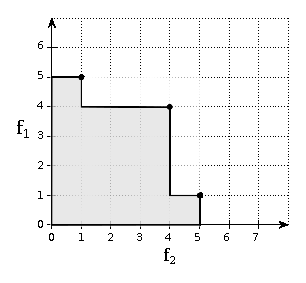
\includegraphics[width=0.3\textwidth]{img/sce/hypervol2}
  \caption{Exemplo de conjunto Pareto bi-objetivo possuindo 18 unidades hiper-volume (área).}
  \label{img:hvol2}
\end{figure}

Visando validar a qualidade do algoritmo SCE, a Tabela~\ref{tab:zitzler} apresenta os
resultados alcançados pelas heurísticas expressos em porcentagem média de hiper
volume alcançado, em relação ao maior hiper-volume de solução conhecida para a instância.
Cada célula apresenta a média de 30 execuções.
Em destaque estão os melhores valores de hiper-volume.
\begin{table}[]
  \centering
  \begin{tabular}{cc|c|c|c|c|c}
  \hline
  { m} &
  { n} &
  { SPEA2} &
  { NSGA-II} &
  { MOEA/D} &
  { MOFPA} &
  { SCE} \\ \hline
  \multirow{2}{*}{2} & { 250} & 90.4 & 86.3 & 96.9 & \textbf{97.8} & 93.6 \\ \cline{2-7}
   & { 500} & 87.6 & 81.7 & 96.9 & \textbf{97.8} & 92.7 \\ \cline{2-7}
   & { 750} & 85.9 & 79.2 & 98.4 & \textbf{99.2} & 92.3 \\ \hline
  \multirow{2}{*}{3} & { 250} & 83.3 & 77.4 & 99.0 & \textbf{99.7} & 89.4 \\ \cline{2-7}
   & { 500} & 72.8 & 65.9 & 92.9 & \textbf{93.6} & 79.4 \\ \cline{2-7}
   & { 750} & 77.5 & 73.3 & 94.7 & \textbf{95.2} & 79.8 \\ \hline
\end{tabular}

  \caption{Hiper-volume médio alcançado por cada heurística.}
  \label{tab:zitzler}
\end{table}

Pode-se observar pela Tabela~\ref{tab:zitzler} que, apesar de não apresentar resultados
melhores que os do MOEA/D e que os do recente MOFPA,
os resultados alcançados pelo SCE foram consistentes,
sendo melhores que as heurísticas SPEA2 e NSGA-II.

\missingf{Tem que aprofundar essa discussão: porque o SCE foi superior e inferior a cada metaheuristica? Será que as melhores usam mais conhecimento especifico do problema do que as outras?

\resp 
Nenhuma delas usa conhecimento específico. Aliás, o NSGA-II, o SPEA-II e o MOEA/D são heurísticas genéricas.
Apenas a proposta do MOFPA foi dedicada ao MOKP, ainda assim não utiliza nenhum conhecimento específico, é só uma proposta de PSO+Firefly
que testaram no MOKP.
Nem no artigo do MOFPA encontrei alguma indicação de porque ficou melhor que as outras.
Seria mesmo interessante explicar por que são melhores, mas estou achando difícil. Não sei o que dizer.
}

A utilização da \kdtree{} foi comparada à utilização da lista encadeada,
por ser a estrutura utilizadas nos algoritmos heurísticos em questão.
A Tabela~\ref{tab:scecpu} apresenta o tempo computacional médio demandado pela execução do
algoritmo SCE para cada uma das 6 instâncias para a utilização da Lista encadeada,
\dtree{2} e, no caso 3-objetivo, \dtree{3}.
A coluna $\ndcol$ apresenta o tamanho médio do conjunto Pareto aproximado dado como
resposta pelo algoritmo.

\missingf{Porque usou lista e nao avl? No exato usou AVL. Porque mudou? Tem que justificar.

\resp Como o objetivo dos testes era comparar a utilização da \kdtree{} com o que a literatura utiliza,
eu utilizei apenas a lista no caso heurístico.
A AVL eu só utilizei no exato por ter sido a proposta da Bazgan para o algoritmo exato.
Adicionei essa explicação ao texto.
}

\begin{table}[]
  \centering
  \begin{tabular}{crr|r|rr|rr}
  \hline
  %%%%%%%%%%%%%%%%%
  %   HEADER
  %%%%%%%%%%%%%%%%%
  \multicolumn{3}{c|}{Instância}
  & \multicolumn{1}{c|}{Lista}
  & \multicolumn{2}{c|}{\dtree{2}}
  & \multicolumn{2}{c}{\dtree{3}}
    \\
  $\np$
  & $n$ \phantom{a}
  & $\ndcol$
  & tempo (s)
  & tempo (s)
  & speedup
  & tempo (s)
  & speedup
    \\ \hline
\multirow{2}{*}{2}
 & 250 &  88.4 & \textbf{  9.3} & 13.1 & 0.71 & -- & -- \\ \cline{2-8}
 & 500 & 106.0 & \textbf{ 14.3} & 18.3 & 0.78 & -- & -- \\ \cline{2-8}
 & 750 & 120.4 & \textbf{ 18.7} & 22.3 & 0.84 & -- & -- \\ \hline
\multirow{2}{*}{3}
 & 250 & 705.5 &  9.8   & 10.1 & 0.97 & \textbf{  9.1} & 1.08 \\ \cline{2-8}
 & 500 & 672.8 & 15.6   & 16.0 & 0.98 & \textbf{ 15.2} & 1.03 \\ \cline{2-8}
 & 750 & 646.0 & 22.0   & 24.2 & 0.91 & \textbf{ 21.8} & 1.01 \\ \hline
\end{tabular}

  \caption{Tempo computacional médio do algoritmo SCE para instâncias Zouache.}
  \label{tab:scecpu}
\end{table}

A Figura~\ref{fig:cmpsce} apresenta o número médio de avaliações de solução
para os casos (a) bi-objetivo e (b) 3-objetivo.
O eixo horizontal refere-se ao tamanho da instância (número de itens)
enquanto que o eixo vertical refere-se ao número médio de avaliações de solução.

\missingf{Vc usou várias vezes "numero medio de avaliação de soluções" e agora usou "numero medio de avaliações de solução". 
Favor uniformizar ao longo do texto do capítulo. Eu prefiro "numero medio de avaliações de solução"

\resp Ok. Uniformizei assim.}

\begin{figure}
\centering
\begin{subfigure}{.5\textwidth}
  \centering
  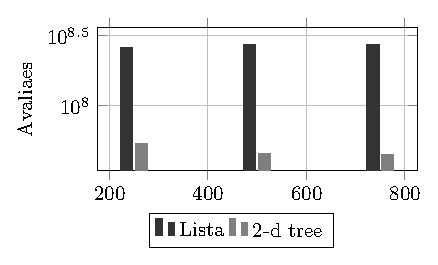
\includegraphics[scale=1.1]{tab/sce/cmpres2}
  \caption{Instâncias 2-objetivo}
  \label{fig:cmpsce2}
\end{subfigure}%
\begin{subfigure}{.5\textwidth}
  \centering
  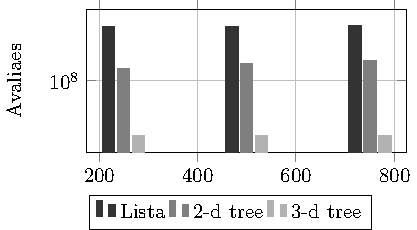
\includegraphics[scale=1.1]{tab/sce/cmpres3}
  \caption{Instâncias 3-objetivo.}
  \label{fig:cmpsce3}
\end{subfigure}
\caption{Número de avaliações médio do algoritmo SCE para instâncias Zouache.}
\label{fig:cmpsce}
\end{figure}

Pode-se observar que a \dtree{2} não foi capaz de oferecer melhoria no tempo computacional
demandado pelo algoritmo, apesar da redução no número de avaliações de solução.
Este resultado se deve ao tamanho reduzido do conjunto Pareto mantido pelo algoritmo,
em especial para os casos bi-objetivo.
Para os casos 3-objetivo ainda se pode observar um pequeno speedup no
caso da \dtree{3}, devido a se ter maiores conjuntos Pareto,
o que não torna favorável o \emph{overhead} adicional da estrutura.

\missingf{Interessante expandir mais a dicussao do porque o resultado nao foi bom!

\resp Complementei apontando o problema do overhead. (no parágrafo abaixo eu continuo a discussão) }

Vale também observar que, para o algoritmo heurístico,
a demanda de operações de verificação
de dominância é relativamente pequena em relação às outras operações relacionadas
ao caráter evolucionário do algoritmo, diferentemente do algoritmo exato,
cujo desenvolvimento se baseia em sua maioria na operação de verificação de dominância,
o que também explica o insucesso da \kdtree{} nesse caso.
